\chapter{Monitorowanie procesu gojenia ścięgna Achillesa}
\section{Ścięgno Achillesa}
Ścięgno Achillesa, nazywane również ścięgnem piętowym, jest największym i najsilniejszym ścięgnem występującym w ciele ludzkim. Stanowi wspólne zakończenie mięśnia trójgłowego łydki, w którego skład wchodzą dwie głowy mięśnia brzuchatego i mięsień płaszczkowaty. Całość struktury zlokalizowana jest w tylnym, powierzchownym przedziale łydki, co zostało przedstawione na Rysunku \ref{muscle_structure}.  
\begin{figure}[h!]
\centering
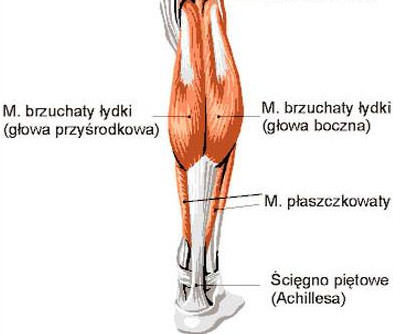
\includegraphics[width=0.55\textwidth]{figures/muscleStructure.jpg}
\caption{Lokalizacja mięśnia trójgłowego łydki wraz ze ścięgnem Achillesa.}
\label{muscle_structure}
\end{figure}
Z obu głów (brzuścców) mięśnia brzuchatego łydki wyrasta jedno szerokie, płaskie ścięgno, które jest początkiem części brzuchatej ścięgna Achillesa. Następnie ścięgno to łączy się z włóknami pochodzącymi od mięśnia płaszczkowatego, które układają się stycznie do wcześniej powstałej struktury. Wówczas kształt ulega stopniowemu zwężeniu i zaokrągleniu, aż do punktu o minimalnej szerokości (około 4 cm nad przyczepem dolnym [1]). W rejonie samego przyczepu dolnego znajdującego się na tylnej powierzchnia kości piętowej, ścięgno ponownie jest płaskie i szerokie.

W kolejnych podsekcjach szczegółowo omówiona została anatomia ścięgna Achillesa, jego biomechanika, potencjalne urazy wraz z czynnikami im sprzyjającymi oraz proces gojenia i możliwości jego wspomagania. Wszystkie te aspekty są istotne z uwagi na możliwości monitorowania procesów fizjologicznych występujących w ścięgnie. 
\subsection{Anatomia}
Średnia długość ścięgna Achillesa to 15 cm (11 - 26 cm). Średnia szerokość w rejonie początku wynosi 6.8 cm (4,5 - 8, 6 cm). Następnie, stopniowo ścięgno ulega zwężeniu do punktu o minimalnej szerokości 1.8 cm (1,2 - 2,6 cm). W rejonie samego przyczepu struktura ponownie się rozszerza i jej szerokość wynosi średnio 3.4 cm (2,0 - 4,8 cm) [2-3].

ścięgno jest zbudowane z tkanki łącznej, dokładniej tkanki łącznej właściwej zbitej. Składa się z komórek takich jak fibroplasty, komórki tuczne, komórki plazmatyczne, histiocyty i komórki napływowe oraz z \textit{istoty międzykomówrkowej}, substancji wypełniającego. W skład istoty międzykomórkowej (nazywanej też \textit{macierzą międzykomórkową}) wchodzi istota podstawowa (ang. \textit{ground substance}) oraz włókna. Istota podstawowa jest rodzajem żelu wiążącym duże ilości wody i włókna, których można z kolei wyróżnić trzy rodzaje: kolagenowe, siateczkowe i sprężyste.

Włókna kolagenowe i siateczkowe są zbudowane z fibrylarnego białka -- kolagenu, najczęściej występującego białka w organizmie człowieka, stanowiącym około 25\% wszystkich białek. Makrocząsteczki kolagenu składają się ze zwiniętych łańcuchów polipeptydowych tworzących helisy. Dotychczas zidentyfikowano 20 typów kolagenu różniących się od siebie szczegółową budową helisy. Kolagen typu I stanowi około 90\% wszystkich pozostałych typów i jest podstawowym budulcem włókien kolagenowych występujących zazwyczaj w wiązkach, o grubości 50--100$\mu$$m$. Włókna siateczkowe zbudowane są natomiast w przeważającym stopniu z kolagenu typu III. Pozostałe typy kolagenu występują w znacząco mniejszym stopniu tworząc włókienka różnej grubości od 10 do 300 nm (por. [Hist]).

Włókna sprężyste występują w postaci sieci i mają średnicę 0,2--10 $\mu$$m$. Zbudowane są z elastyny, rozciągliwego i sprężystego białka. Dzięki temu włókna sprężyste pod wpływem działania siły zewnętrznej mogą zwiększać swoją długość nawet o 50\% (za. [Hist]). 

ścięgno Achillesa składa się ze ściśle upakowanych włókien sprężystych i kolagenowych, głównie typu I.  Włókna kolagenowe stanowią 70\% masy suchego ścięgna i charakteryzują się hierarchiczną strukturą zobrazowaną na Rys. \ref{Achilles-histology}  
\begin{figure}[h!]
	\centering
	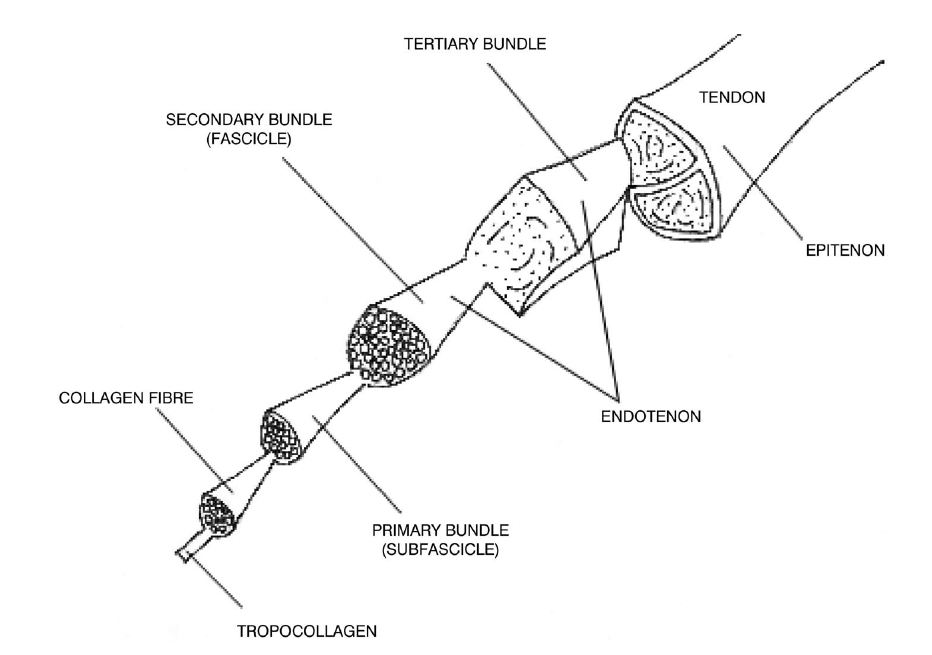
\includegraphics[width=0.8\textwidth]{figures/Achilles_hist.png}
	\caption{Schemat hierarchicznej budowy ścięgna Achillesa.}
	\label{Achilles-histology}
\end{figure}
W skład ścięgna wchodzą: włókna, wiązki pierwszo, drugo i trzeciorzędowe oraz ościęgno [model-17]. 

ścięgno zawiera niewiele istoty podstawowej jak i komórek (zob. [model-14]). Istota podstawowa stanowi otoczkę włókien zapewniając możliwość transportu wody i substancji odżywczych [model-17]. Komórki natomiast są poukładane w wąskie pasy leżące pomiędzy włóknami kolagenowymi [model-14]. 

W przeciwieństwie do innych ścięgien, ścięgno Achillesa nie posiada pochewki ścięgnistej, lecz jest otoczone ościęgnem utworzonym z tkanki łącznej włóknistej. Struktura ta jest bogata w naczynia krwionośne i jest bardzo ważnym elementem w procesie gojenia. Oprócz otaczającej tkanki łącznej ścięgno czerpie źródło unaczynienia z brzuśców mięśni brzuchatego i płaszczkowatego oraz z połączenia kostno-ścięgnistego. Najsłabsze unaczynienie występuje poziomie ok. 4-5 cm powyżej górnego brzegu kości piętowej (por. [Bochenek]).

W połowie długości między kostką przyśrodkową, a ścięgnem, pomiędzy blaszką powierzchowną i głęboką rozcięgna zginaczy, biegnie nerw piszczelowy. W pobliżu ścięgna przebiega też nerw łydkowy, który krzyżuje się ze ścięgnem w odległości 8,7-12,4 cm proksymalnie od guza piętowego, biegnie w dół i na wysokości guza znajduje się około 11 mm bocznie i 18 mm grzbietowo od niego (por. [Bochenek]). 

\subsection{Biomechanika}
\label{Biomechanika}
Zadaniem ścięgien jest transfer siły mięśniowej do układu szkieletowego. Pod względem mechanicznym ścięgno piętowe jest najsilniejszym ścięgnem całego ustroju. Wytrzymuje obciążenia wahające się nawet do 300 kg, w badaniach eksperymentalnych wykazano, że do przerwania zdrowego ścięgna Achillesa potrzebna jest siła przekraczająca 400 kg [Etiologia-2,16,23]. Dla przykładu podczas chodu maksymalne obciążenie ścięgna Achillesa wynosi 500 N, przy biegu jest to 9000 N, natomiast podczas wyskoku może sięgać 12000 N. Podobne obciążenia wytrzymuje tylko ścięgno właściwe rzepki [Etiolo 1,24].

Głównym zadaniem ścięgna Achillesa w trakcie prawidłowego chodu ma nieocenione znaczenie, w dużym stopniu odpowiada za ruch zginania podeszwowego stopy, co wiążę się ze zwiększonym ryzykiem nadmiernego napięcia, a w konsekwencji do przeciążenia, rozwoju stanu zapalnego, a nawet uszkodzenia [Etiologia-1,19].

Obciążenia te są implikacją głównego zadania ścięgna piętowego, czyli odpowiedzialności za \textit{zginanie podeszwowe stopy}, a zatem za wyprost powodujący np. wspięcie na palce. Cały proces rozpoczyna się od centralnego układu nerwowego skąd wysyłane są impulsy nerwowe. Trafiają one do odpowiednich grup mięśniowych za pośrednictwem \textit{nerwu ruchowego}, który przewodzi impulsy wzbudzając proces skurczu mięśni. Na styku nerwu z mięśniem znajduje się \textit{synapsa nerwowo-mięśniowa} (tzw. \textit{płytka motoneuronalna}). Do niej właśnie na skutek impulsu wydzielany jest neuroprzekaźnik, \textit{acetylocholina}, na skutek czego następuje dalsze pobudzenie błony komórki mięśniowej i uwolnienie jonów wapnia Ca$^{2+}$. Jest to kluczowy składnik implikujący skurcz mięśni. Cały proces pobudzeń, trwający dla mięśni szkieletowych 100--300 milisekund przedstawiono na Rys. \ref{muscle-excitements} 
\begin{figure}[h!]
	\centering
	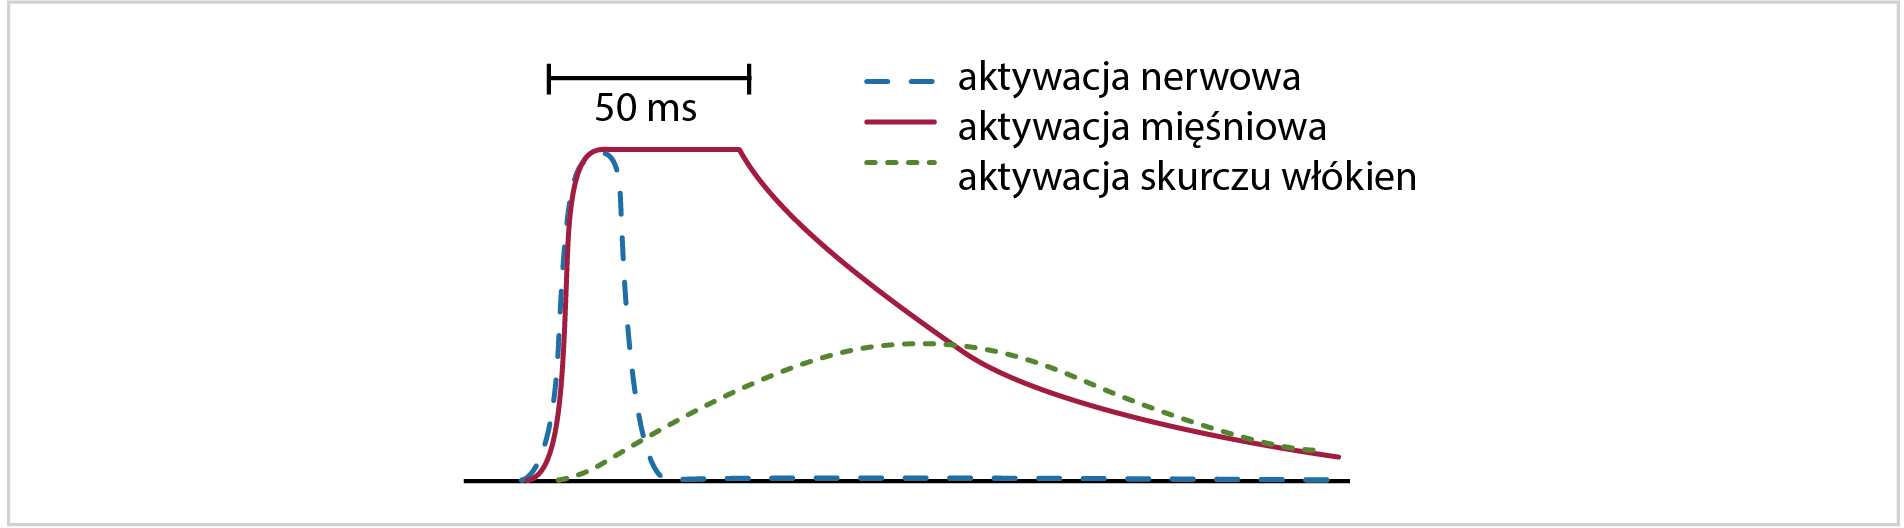
\includegraphics[width=0.6\textwidth]{figures/skurcz_miesni.png}
	\caption{Schemat generowania skurczu mięśni.}
	\label{muscle-excitements}
\end{figure}

Skurcz generuje siłę, która jak wcześniej opisano, przekazywana jest za pomocą ścięgien do układu szkieletowego. Dobrym przybliżeniem tego procesu jest \textit{model Hill'a} [], którego schemat przedstawiono na Rys. \ref{hill-model}.

\begin{figure}[h!]
	\centering
	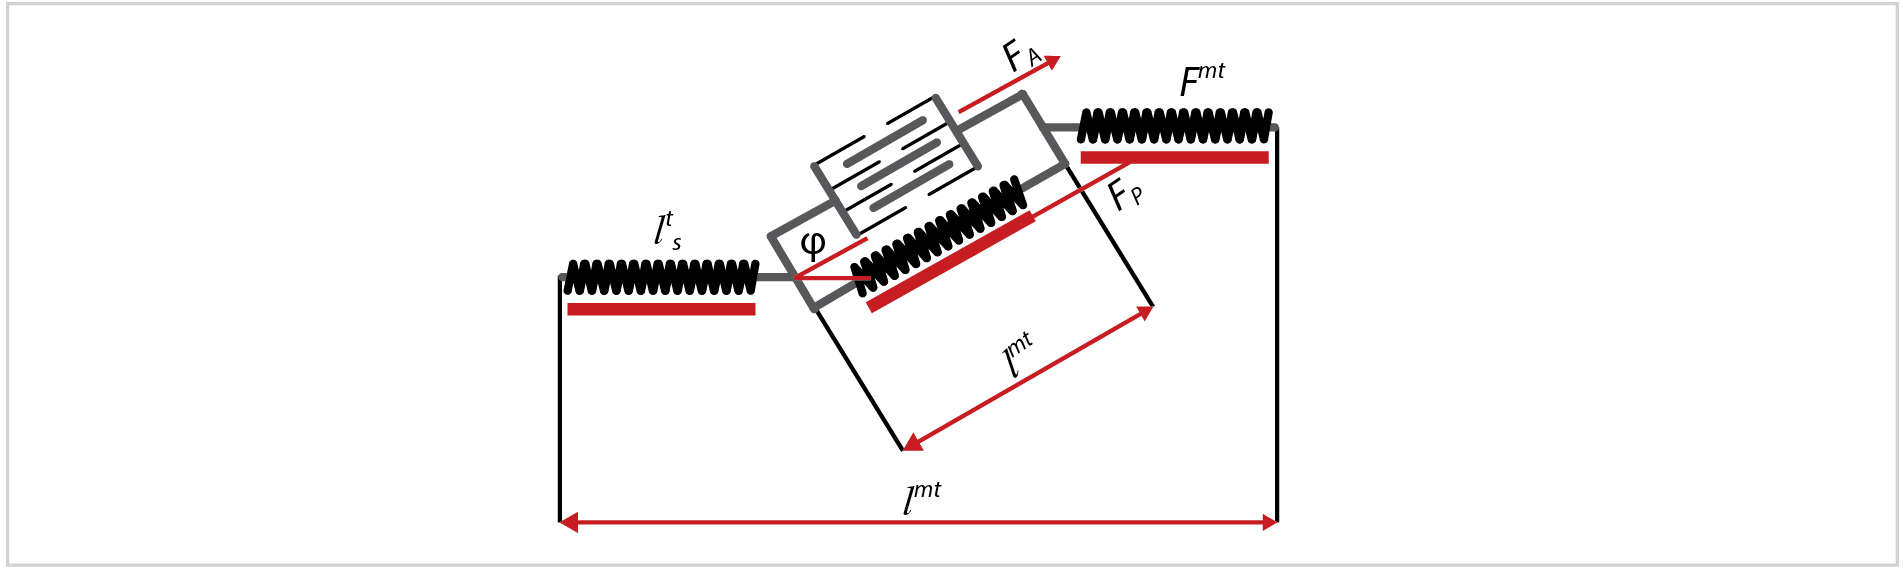
\includegraphics[width=0.6\textwidth]{figures/Hill.png}
	\caption{Schemat modelu Hilla.}
	\label{hill-model}
\end{figure}

$F_A$ oznacza siłę aktywnie wywoływaną skurczem mięśni, $F_P$ to pasywna siła odpowiadająca za bezwładność tkanki miękkiej w mięśniu, a $F^{mt}$ to wynikowa siła przekazywana przez ścięgno, która zależy od długości ścięgna $l_t$ i kąta $\phi$ pomiędzy ścięgnem a mięśniem. To właśnie na skutek przekroczenia wartości granicznej siły $F^{mt}$ dochodzi najczęściej do urazu ścięgna Achillesa. Dokładny opis tego problemu wraz z jego implikacjami został przedstawiony w kolejnej podsekcji.

\subsection{Urazy i czynniki im sprzyjające}
\subsection{Leczenie, fazy gojenia i rehabilitacja}
\label{gojenie}
/*farmakologia*/
/* fizjoterapia */
/* fizykoterapia - fala, amplituda, częstotliwość*/ 

 Nevertheless, the stages of tendon healing are similar to those of other connective tissues, i.e. there are three consecutive,
however overlapping phases: i) in
ammatory; ii) proliferative or reparative; and iii)
remodeling phase [model-17, 21, 6]

The in
ammation begins immediately after the accident. At the site of the in-
jury blood clot begins to form and starts to activates the release of pro-in
ammatory
chemicals that, in turn, causes an in
ux of 
uids and in
ammatory cells from the
surrounding tissue [model-13]. In
ammatory cells engage in the phagocytosis of devi-
talised tissue and debris and break down the hemorrhage and clot [model-21, 3, 13]. At
that time, the recruitment and activation of tenocytes begins, however peaks in the
next, proliferative stage [model-21].
The next, proliferative phase, begins roughly two days after the injury [model-21].
Tendon cells continue to migrate and proliferate about the injury site and start to
produce new collagen bers (type III) that are more randomly oriented [model-21, 3, 6].
The level of some in
ammatory cells start to decline. At the same time, other
in
ammatory cells such as macrophages continue to release growth factors that
activate and direct tenocytes recruitment towards injury site [model-21].
The last, remodeling phase begins after one or two months after the injury
[model-21]. At that time, the type III collagen bers are replaced with type I collagen
bers that are also reoriented and aligned in the direction of stress [model-21]. After
about six weeks till about ten weeks after the injury reconstructed tissue changes
from cellular to brous [model-17]. The remodeling phase of tendon healing may last as
long as eighteen months and even surgically repaired tendons never return to full
strength. 

\section{Zastosowanie rezonansu magnetycznego}
Obrazowanie metodą \textit{Magnetycznego Rezonansu}, w skr. \textit{MR} (ang. \textit{Magnetic Resonance Imaging}, w skr. \textit{MRI}) jest metodą bazującą na odpowiednim odczycie reakcji atomów na silne pole magnetyczne. Zrozumienie tych procesów było efektem prac związanych z mechaniką kwantową takich jak: Einstein, Edwin Shrodinger, Heisenberg czy Pauli /*uzupełnij z licznych książek - krótką historię*/. Wymienione prace z początku XX wieku umożliwiły rozwój technologii MR zainicjowane zrozumieniem w latach 30-tych magnetycznej natury \textit{protonów}, cząstek subatomowych, które wraz z \textit{neutronami} wchodzą w skład jądra atomowego (zob. [1933 - stern gerlach]).

Dokładniej rzecz biorąc, główną własnością jądra atomowego umożliwiającą działanie MR jest \textit{spin}. Można powiedzieć, że jądro posiada spin jeżeli nie ma jednocześnie parzystej liczby protonów i parzystej liczby neutronów (por. [Rezonans magnetyczny]). Jądra o parzystej liczbie atomowej mają w \textit{stanie podstawowym} (charakteryzującym się najniższą energią) spin całkowity, a o nieparzystej połówkowy.

Cząstki o niezerowym spinie pochłaniają fale elektromagnetyczne o specyficznej częstotliwości konwertując energię na ruch rotacyjny nazywany \textit{rezonansem magnetycznym}. Zjawisko to opisuje się równaniem Larmora \ref{MRLarmor}:
\begin{equation}
\label{MRLarmor}
\omega_0 = \gamma \ast \beta_0,
\end{equation}
gdzie $\omega_0$ to prędkość obrotowa protonów (tzw. częstotliwość Larmora), $\gamma$ to współczynnik żyromagnetyczny właściwy danemu protonowi, a $\beta_0$ to wartość zadanego pola magnetycznego. Dla przykładu częstotliwość Larmora dla protonu wodoru, gdzie $\gamma$=42,57 MHz/T dla pola 1,5T równa jest 63,8 MHz. Wodór jest najczęściej wykorzystywanym pierwiastkiem w metodzie rezonansu magnetycznego, gdyż jest obecny w 99,98\% ludzkich tkanek (za [MR]). Jednak w szczególnych przypadkach stosuje się również obrazowania z wykorzystaniem częstotliwości odpowiednich dla fosforu, sodu czy węgla (zob. []).

Rezonujące protony mają własności podobne do magnesów prętowych i mogą być ukierunkowane przy pomocy pola magnetycznego. Protony o wysokich poziomach energii odchylają się przeciwnie do kierunku zadanego pola magnetycznego tzw. \textit{protony antyrównoległe}, a o niskich poziomach energii odchylają się zgodnie z kierunkiem pola tzw. \textit{protony równoległe}. W przeciętnym wycinku ciała ludzkiego jest więcej protonów równoległych niż antyrównoległych. Przykładowo w objętości 1 $\times$ 1 $\times$ 5 mm jest to liczba około 2 $\times$ $10^15$ cząstek. Różnica ta tworzy całkowitą magnetyzację $M_0$ danego obszaru.

Przy pomocy sterowanych impulsów o częstotliwości fal radiowych (tzw. $impulsy RF$) wykonywana jest zmiana $M_0$ obszaru, tworząca sygnał MR. Impulsy RF zawierają przestrzennie zmieniające się pole magnetyczne różnicujące częstotliwość i fazę precesji protonów, co wykorzystywane jest do kodowania lokalizacji przestrzennej $x$, $y$ sygnału. Kodowanie warstwy $z$ odbywa się na podstawie ustawiania częstotliwości Larmora dla danego obszaru.

Nieprzetworzona informacja z kierunków $x$, $y$, $z$ nazywana jest \textit{przestrzenią K} i koduje ona składniki częstotliwości sygnału. Do transformacji z przestrzeni częstotliwości na przestrzeń obrazu używana jest operacja matematyczna zwana \textit{odwrotną transformacją Fouriera}. Przykład takiego działania można znalexć w [http://mriquestions.com/fourier-transform-ft.html].

Z uwagi na różne parametry mierzone w reakcji protonów na zadane pole magnetyczne powstało wiele \textit{sekwencji MR} oraz ich składowych nazywanych w tej pracy \textit{protokołami MR}. Do badań opisanych w dalszej części tego manuskryptu zostało użytych 10 często stosowanych wariantów pracy rezonansu magnetycznego. Zostaną one pokrótce scharakteryzowane poniżej:
\begin{itemize}
	\item \textit{T1} -- mierzona jest \textit{relaksacja T1}, a zatem czas potrzebny protonom na powrót do stanu początkowego po odchyleniu o 90$^\circ$. Sygnał rezonansu magnetycznego $MR_s$ można obliczyć z zależności:
	\begin{equation}
		MR_s \sim \gamma_{pd} \ast [1-e^{-TR/T1}],
	\end{equation}
	gdzie $\gamma_{pd}$ to gęstość protonowa tkanki, $TR$ to \textit{czas repetycji} określany przez użytkownika.
	\item \textit{T2} -- mierzona jest \textit{relaksacja T2}, tj. czas potrzebny do utraty spoistości pomiędzy między spinami. Dokładniej mówiąc mierzone są różnice w częstotliwości Larmora powstające w czasie, wynikające z umiejscowienia protonów w różnych ośrodkach i niejednorodności w pobudzeniach polem magnetycznym. $MR_s$ przyjmuje wówczas następującą zależność:
	\begin{equation}
	\label{T2ecquation}
	MR_s \sim \gamma_{pd} \ast [1-e^{-TE/T2}],
	\end{equation}
	gdzie $TE$ to \textit{czas echa} zdefiniowany przez użytkownika.
	\item \textit{PD} (od ang. \textit{Proton Density}) -- mierzona jest gęstość spinowa tkanki wprost proporcjonalna do liczby protonów. Wówczas:
	\begin{equation}
	MR_s \sim \gamma_{pd}.
	\end{equation}
	\item \textit{T2 mapping} -- $T2$ z sygnału \ref{T2ecquation} mierzona jest dla wielu $TE$, co pozwala na interpolacje między wynikami z własnym doborem parametrów (zob. [Regulski]).
	\item \textit{T2 $^\ast$ GRE} (od ang. \textit{Gradient Echo}) -- w sekwencjach gradientowych protony odchylane są o kąt mniejszy od $90^\circ$ (zazwyczaj 10$^\circ$ -- 80$^\circ$). Odchylenia protonów występują w sekwencji prowadząc do cyklicznego przefazowania spinów. Dzięki temu uzyskuje się skupione echo gradientowe w czasie $TE$, w którym sygnał $MR_s$ jest zależny od obu czynników $T1$ i $T2$:
	\begin{equation}
	MR_s \sim \gamma_{pd} \ast [1-e^{-TE/T2}][1-e^{-TR/T1}],
	\end{equation}
	przy czym dla mniejszych kątów wkład $T2$ rośnie w stosunku do wkładu $T1$.
	\item \textit{T2 $^\ast$ GRE TE\_MIN} (od ang. \textit{Minimal Time Echo}) -- mierzone jest $T2$ z sygnału \ref{T2ecquation} przy minimalnym czasie $TE$ i tylko dla fragmentu przestrzeni K. 
	\item \textit{3D FSPGR} (od ang. \textit{Fast Spoiled Gradient Echo}) -- jest to szybka sekwencja gradientowa, wykorzystująca echo szczątkowe oraz \textit{spoiler}, tj. metodę do rozbicia wszelkiej pozostałej magnetyzacji na końcu każdego cyklu przefazowania. W tej pracy użyto czterech protokołów tej sekwencji. Wszystkie bazują na różnicy w częstotliwościach rezonansowych protonów wchodzących w skład tłuszczu i wody. Dokładniej:
	\begin{itemize}
		\item In Phase Ideal -- sygnał mierzony w czasie, gdy protony należące do tłuszczu i wody są w zgodnej fazie;
		\item Out Phase Ideal -- sygnał mierzony w czasie, gdy protony należące do tłuszczu i wody są w antyfazie;
		\item Fat Ideal -- sygnał mierzony przy maksymalnej fazie protonów tłuszczu i minimalnej protonów wody;
		\item Water Ideal -- sygnał mierzony przy maksymalnej fazie protonów wody i minimalnej protonów tłuszczu.
	\end{itemize}
\end{itemize}

Zdecydująca część protonów wodoru znajduje się w tkankach miękkich człowieka dlatego rezonans magnetyczny może być wykorzystany do monitorowania gojenia się ścięgien i więzadeł. W szczególności obserwowana jest ciągłość ścięgna w płaszczyznie sagitalnej, uszkodzenia śródścięgniste objawiające się przerwaniem w naturalnym warkoczu ułożonym z tkanek, pogrubienia ścięgna w szczególności oceniane w przekrojach axialnych jednorodność wrzecionowatość i inne nieregularności kształtu, ostrość ścięgna i jego rozgraniczenie od tkanek otaczających i zmiany na brzegach, obrzęk w okalających ścięgno tkankach, jednorodność charakteryzująca się podobieństem przekrojów sąsiednich, liczbę ewentualnych zrostów.

\section{Zastosowanie ultrasonografii}

Kolejną z metod obrazowania medycznego jest \textit{Ultrasonografia}, w skr. \textit{USG} (ang. \textit{Ultrasonography}, \textit{US}). Bazuje ona na efektach związanych z propagacją w tkankach \textit{ultradźwięków}, tj. fal akustycznych o częstotliwościach powyżej 20 kHz.

Propagacja fal w przyrodzie była tematem rozważań myślicieli takich jak Pitagoras, Arystoteles czy Galileusz, którzy ugruntowali pole badań pod kolejne osiągnięcia matematyczno-inżynieryjne. W tej kwestii, do jednego z przełomów doszło w 1822 roku, kiedy to szwajcarski inżynier Daniel Colladen oraz matematyk Charles-Francois Sturm wyznaczyli przybliżoną prędkość rozchodzenia się fali akustycznej w wodzie. Badanie wykonano na Jeziorze Genewskim symultanicznie mierząc czas jaki potrzebny był dźwiękowi podwodnego wystrzału i sygnałowi dzwonka rozchodzącego się w powietrzu do przebycia drogi pomiędzy dwoma łódkami oddalonymi o 10 mil. Wyliczona wartość wyniosła wówczas 1435 m/s nie różniąc się znacząco od dzisiaj przyjmowanej estymacji równej 1480 m/s. Analogicznie wyliczane są obecnie prędkości rozchodzenia się w fali w innych ośrodkach takich jak powietrze, tkanki miękkie, kości itp.

58 lat później, w 1880 roku bracia Curie opisali w \cite{Curie1880} \textit{efekt piezoelektryczny}, czyli zjawisko polegające na pojawieniu się ładunku elektrycznego pod wpływem naprężeń mechanicznych w krysztale o anizotropowej budowie, takiej jak ma np. kwarc. W przypadku odwrotnym, przyłożenie napięcia do odpowiedniego kryształu generuje drgania. 

Efekty te są wykorzystywane w \textit{głowicy aparatu usg}, przyrządu do generowania i odbierania ultradźwięków. Przykładowo, polaryzowanie kryształu piezoelektrycznego krótkim impulsem elektrycznym $\sigma_1(t)$ pobudza go do drgań na własnej częstotliwości rezonansowej. Zakładając, że kryształ ma kształt walca o grubości $d$=0,64mm, to będzie stanowił rezonator półfalowy, w którym wystąpi drganie rezonansowe o długości fali $\lambda = 2d$ czyli $\lambda = 1,28$ mm. Jeżeli wykonany jest z tytanianu baru, dla którego prędkość propagacji drgań wynosi $c$=4460m/s, to częstotliwość drgań własnych tego
kryształu wyniesie:
\begin{equation}
f = \frac{c}{\lambda} = \frac{4460 m/s}{1,28 mm} = 3,5 MHz.
\end{equation}
Odwrotnie, powracająca fala tzw. \textit{echo} wygeneruje impuls elektryczny $\sigma_2(t)$ w skutek drgań wywołanych w krysztale. 
 
Echo jest naturalnie falą różniącą się od sygnału nadawanego, a zmiany te są w przeważającym stopniu efektem zjawisk znanych z optyki falowej tj. \textit{odbicia}, \textit{załamania}, \textit{dyfrakcja}, \textit{rozpraszanie} i \textit{pochłanianie} (zob. []).

Zależą one on częstotliwości fali, która propaguje się w ośrodku o pewnej \textit{impedancji akustycznej ośrodka} $Z$ wyrażanej jako:
\begin{equation}
Z = \rho c = \sqrt{\epsilon \rho},
\end{equation}
gdzie $c$, to prędkość rozchodzenia się fali, $\rho$ to gęstość ośrodka, a $\epsilon$ to \textit{moduł odkształcalności objętościowej}, tj. parametr opisujący jak zmieni się objętość ośrodka pod danym ciśnieniem. Parametry wybranych ośrodków zestawiono w Tabeli \ref{USG-params} 
\begin{figure}[h!]
	\centering
	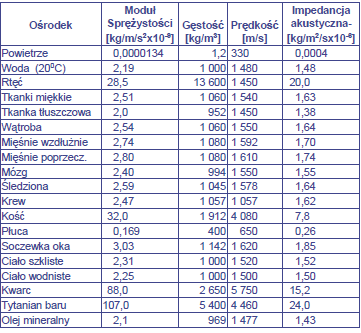
\includegraphics[width=0.55\textwidth]{figures/USG-params.png}
	\caption{Parametry ośrodków często mierzonych w badaniach USG.}
	\label{USG-params}
\end{figure}

Dla przykładu, do zjawiska załamania lub odbicia dochodzi kiedy fala pada na granice dwóch ośrodków o różnych impedancjach akustycznych $Z_1$ i $Z_2$. Zależność ta opisana jest prawem Snella:
\begin{equation}
R = \frac{I_r}{I_0} = \left(\frac{Z_1-Z_2}{Z_1+Z_2}\right)^2,
\end{equation}
gdzie $I_r$ to natężenie fali padającej, a $I_0$ odbitej. Natomiast $R$, czyli współczynnik odbicia, jest parametrem, który rośnie wraz ze wzrostem kąta odchylenia od kierunku prostopadłego, aż do całkowitego odbicia.

Z kolei do rozpraszania bądz pochłaniania fali dochodzi kiedy to fala pokonuje daną drogę w ośrodku o pewnej $Z$, co zapisywane jest następująco:
\begin{equation}
I=I_0 \epsilon^{-\gamma x},
\end{equation}
gdzie $\gamma$ to współczynnik osłabienia zależny od $Z$, a $x$ to droga przebyta przez falę. Efekt ten można korygować poprzez dobór odpowiedniego $I_0$.

Analiza amplitudy i częstotliwości sygnału nadanego i echa umożliwia rekonstrukcję obrazu USG. W przypadku najczęściej stosowanych w praktyce rekonstrukcji przekrojów dwuwymiarowych (tzw. tryb B) współczesny tor budowania prezentacji wizualnej (tzw. \textit{beamforming}) wygląda następująco: 
\begin{enumerate}
	\item Głowica ultradźwiękowa emituje impulsy w postaci wąskiej wiązki w ściśle określonym kierunku. Wiązka zawiera sygnał z $N$ przetworników zawierających kryształy piezoelektryczne.
	\item Echa z danego kierunku pozwalają na obliczenie pojedynczego promienia akustycznego, który jest iloczynem charakterystyk nadawanego i odbieranego sygnału.
	\item Wszystkie promienie, których we współczesnych aparatach może być do kilkuset (zob. [GE Voluson]), służą do formowania obrazu, który tworzony jest we \textit{współrzędnych biegunowych} ($r$, $\theta$) w przypadku głowic mechanicznych sektorowych, wieloelementowych convex czy fazowych lub we współrzędnych prostokątnych ($x$, $y$) w przypadku głowic mechanicznych lub wieloelementowych liniowych\footnote{szczegółowy opis głowic USG i ich charakterystyk można znalezć w []}. 
\end{enumerate}

Tryb B umożliwia również wizualizację obrazów dynamicznych. Przykładowo jeżeli na obraz składa się 400 promieni i każdy odsłuchiwany jest do głębokości 15cm, to czas gromadzenia danych dla ośrodka o średnim c=1500 m/s wynosi $2\frac{2\times15}{1500 m/s}\times400 = 0,08 s$, czyli 12 obrazów na sekundę. Częstotliwość tę można zwiększać, zmniejszając liczbę promieni lub głębokość obserwacji.

Innym często stosowanym trybem rekonstrukcji obrazu (wykorzystywanym również w tej pracy) jest tryb D bazujący na \textit{efekcie Dopplera}, do którego dochodzi w przypadku przechodzenia fali przez ośrodki względem siebie się przesuwające. Zmienia się wówczas częstotliwość fali, co wyrażone jest następującym wzorem:
\begin{equation}
f_r = 2 f_o\frac{v}{c}\cos(\theta),
\end{equation} 
gdzie $f_r$ to zmiana częstotliwości fali nadawanej $f_0$, zależna od kąta $\theta$ pomiędzy falą i ośrodkiem poruszającym się i prędkościami rozchodzenia się fali w obu ośrodkach tj. $v$ i $c$. Tryb D jest wykorzystywany w praktyce np. do monitorowania przepływu krwi w tkankach. 

W kontekście ścięgna Achillesa tryb B jest użyteczny do obrazowania tkanek miękkich. Przydatna jest zwłaszcza możliwość zobrazowania ukierunkowania struktur włókien ścięgnistych na podstawie czego radiolog może wnioskować o fazie gojenia. Składowa czasowa jest interesująca z perspektywy fizjoterapeuty oceniającego m.in. ślizg w ścięgnie przy wykonywaniu odpowiednich ruchów np. zginania podeszwowo-grzbietowego stopy. Tryb D natomiast może służyć do oceny unaczynienia ścięgna w kolejnych etapach gojenia, które jak wiadomo z sekcji \ref{gojenie} zmienia się w czasie.

W porównaniu do rezonansu magnetycznego USG charakteryzuje się niskimi kosztami aparatury. Uzyskiwane obrazy są jednak trudniejsze w interpretacji, co przekłada się na koszty wyszkolenia kadry. W tym kontekście przydatne mogą okazać się nowe rozwiązania w warstwie sprzętowej i oprogramowania. 

Do pierwszej grupy należy zaliczyć zastąpienie przetworników z piezoelektrykami, przetwornikami budowanymi w technologi MEMS np. cMUT, czy pMUT (zob. [butterfly-http://news.mit.edu/2018/startup-butterfly-network-ultrasound-smartphone-0207]) oraz układy pozwalające przetwarzać surowy sygnał ultradxwiękowy (zob. [us4us]). Do drugiej grupy należą algorytmy sztucznej inteligencji pozwalające wydobyć i zinterpretować interesującą informację z niskiej jakości obrazów (np. zob. [nvidia-keynot-clarisa-project]). 

Badania obrazowe nie są jedynymi, które służą do oceny gojenia się ścięgna Achillesa. W kolejnej sekcji zostały opisane metody oceny biomechaniki, które samodzielnie jak i w połączeniu z analizą obrazową stanowią wartościową informację diagnostyczną.

\section{Zastosowanie badań biomechanicznych}

W poprzednich sekcjach zostały opisane dwie najczęstsze metody monitorowania procesu gojenia się ścięgna Achillesa z udziałem badań obrazowych. Innym podejściem jest \textit{ocena funkcjonalna} bazująca na sprawdzeniu w jakim stopniu dany element (tkanka, narząd, organizm) może realizować swoje zadania. W tym celu często stosuje się ocenę \textit{biomechaniki}. Bada ona właściwości mechaniczne elementów składowych organizmów żywych. 

W przypadku ścięgna Achillesa przykładowe pomiary jego funkcji opisanej w sekcji \ref{Biomechanika} wyglądają następująco:

\begin{enumerate}
	\item \textit{ATRS} (od ang. \textit{Achilles Tendon Total Rupture Score}) -- poziom ograniczenia, z którymi borykają się w następstwie urazu w skali od 0 do 100 [Nilsson-Helander i wsp. 2007, Bąkowski i wsp. 2017].
	\item Pomiar stabilograficzny na platformie dynamometrycznej -- Badania odbywały się boso z oczami otwartymi. Wykonane zostały dwie próby po 30 sekund kolejno na prawej i lewej kończynie dolnej. Następnie pacjent przechodził na kolejną platformę do stabilografii dynamicznej (Biodex Balance System), gdzie miał za zadanie utrzymanie równowagi na niestabilnym podłożu. Wykonano 3 próby po 30 sekund na prawej i potem lewej kończynie dolnej (ustawienie platformy na poziomie 2). Wyniki zostają porównane między kończynami. 
	\item Stabilografia statyczna: pomiar drogi wychylenia środka masy pacjenta w trakcie stania jednonóż na platformie dynamometrycznej [mm].
	\item analiza na ścieżce podometrycznej -- Badano rozkład sił nacisków podeszwowej strony stóp na podłoże. Zebrano pomiar podczas stania swobodnego, wspięć na palce oraz przysiadu boso bez odrywania pięt. Następnie dokonano analizy chodu (3 przejścia) i biegu (5 przebiegnięć) boso oraz w obuwiu sportowym. rotacja podudzia [deg], długość kroków [cm], faza podparcia [\%], faza przenoszenia [\%], max heel force [N] oraz max toe force [N]
	\item Test skoczności i mocy (tzw. siły dynamicznej) kończyn dolnych - wyskoki pionowe z miejsca, wykonywane na platformie dynamometrycznej ("JBA" Zb. Staniak, Polska). Wykonano po dwie próby obunóż oraz na prawej i lewej kończynie dolnej w obuwiu sportowym. W celu pełnego zaangażowania kończyn dolnych zalecono pacjentowi podczas badania aby trzymał ręce na biodrach. Zmierzono moc maksymalną $Pmax$ i średnią $Pm$, maksymalną wysokość uniesienia $hmax$ i obniżenia $k$ środka masy ciała przed odbiciem.
	\item Pomiary maksymalnych momentów sił mięśni zginaczy podeszwowych i grzbietowych stawu skokowego. Ze względu na dwustawową funkcję ścięgna Achillesa badanie przeprowadzono w dwóch pozycjach: z wyprostowanym (ryc.1) oraz zgiętym do 50 stopni stawem kolanowym (ryc.2) [Orishimo i wsp. 2008] w warunkach izometrii i izokinetyki w trzech prędkościach kątowych 60$^\circ$/s (5 powtórzeń), 120$^\circ$/s (8 powtórzeń) oraz 180$^\circ$/s (10 powtórzeń) przy wykorzystaniu urządzenia Humac Norm (USA). Przed badaniem osoba odbywała 5 minutową rozgrzewkę na steperze. Do analizy brano wartości maksymalne pomiarów. Wyniki zostały porównane pomiędzy operowaną a zdrową kończyną dolną. Maksymalne wartości momentu siły mięśni zginaczy podeszwowych i grzbietowych stawu skokowego w warunkach izometrii i izokinetyki w dwóch pozycjach: z wyprostowanym oraz zgiętym do 50 stopni stawem kolanowym [Nm] oraz deficyt pomiędzy operowaną i zdrową kończyną dolną [\%]
\end{enumerate}

Wymienione wyżej badania zostały wdrożone w formie protokołu w placówce Carolina Medical Center (grupa Luxmed) [CMC] i zostały określone przez ortopedów i fizjoterapeutów jako wystarczające do oceny przywracania funkcji ścięgna Achillesa po rekonstrukcji. 

Istnieją jednak możliwości rozszerzenia tak zdefiniowanego podejścia, aż do wersji maksimum, która uwzględniałaby pełne modelowanie układu mięśniowo-szkieletowego. Dane wówczas muszą pochodzić z możliwie dokładnych zsynchronizowanych urządzeń pomiarowych:
\begin{itemize}
	\item \textit{Komputerowa analiza ruchu} (ang. \textit{Motion Capture}) -- narzędzie wykorzystujące systemy czujników do zapisu informacji o zmianach położenia obiektu rejestrowanego np. pacjenta. Do wiodących rozwiązań należy zaliczyć systemy firmy Vicon [] lub BTS [].
	\item \textit{Płyty dynamometryczne} (ang. \textit{Force Plates}) -- narzędzie wykorzystywane do pomiaru sił reakcji podłoża w trzech prostopadłych płaszczyznach. Dzięki temu można określić sumaryczny udział mięśni w generowaniu sił odpowiadających za balans ciała, ruch w danym kierunku oraz przeciwstawianie się sile grawitacji. Do wiodących rozwiązań należą płyty firmy Kistler [].
	\item \textit{Elektromiografia}, w skr. EMG (ang. \textit{Electromyography}) -- narzędzie do pomiaru pobudzeń poszczególnych grup mięśniowych podczas ruchu. Wykorzystywane jest m.in. do określenia rozkładu sił zmierzonych przez płyty dynamometryczne na poszczególne mięśnie.
\end{itemize}

W uzupełnieniu, w zależności od problemu stosuje się dalsze uszczegółowienia modelu mięśniowo-szkieletowego z użyciem np.: wymiarów poszczególnych segmentów ciała (np. goleń, udo, tors) tzw. pomiary antropometryczne; pomiarów maksymalnych sił izometrycznych z użyciem systemów takich jak Biodex; pomiarów geometrii kości mierzonych np. z pomocą Tomografii Komputerowej [] ew. MR; znajdowania lokalizacji przyczepów mięśniowych określanych przy pomocy MR lub USG; wyliczenia środka masy poszczególnych segmentów określanych np. przy użyciu badania DXA (od ang. Double X Ray Absorption); określaniu składu włókien mięśniowych widocznych w USG.

Z uwagi na dużą liczbę możliwych do zmierzenia parametrów, ich integracja odbywa się w modelach komputerowych zaimplementowanych w różnego rodzaju oprogramowaniu do symulacji biomechanicznych. Do najczęściej używanych należą Gait22 [], Gait 20 [] oraz obecnie najbardziej złożony AnyBody full body model []. Historia komputerowo wspomaganego, kompleksowego modelowania biomechaniki ruchu sięga wczesnych lat 90-tych ubiegłego wieku, kiedy to Delp i Loan przedstawili oprogramowanie SIMM [SIMM]. Obecnie SIMM jak również inne oprogramowania komercyjne takie jak: Visual 3D (Cmotion Inc.) [], Anybody (Anybody Technology) [], czy Adams (MSC Software Corp.) [], dostarczają narzędzi do wartościowych symulacji np. chodu [], biegu [] jak również konsekwencji różnych zabiegów chirurgicznych [] i chorób []. Istnieją również narzędzia otwarte, do których należą szeroko wykorzystywany OpenSim [] rozwijany na Uniwersytecie w Stanford, czy też Human Motion [] wywodzący się z instytutu badawczego RIKEN w Japonii.

/*Odwróć kolejność - najpierw opisz kompleksową metodę, a potem protokół CMC*/

Biomechanical simulations are driven by data from mathematical models chosen for the specific application. In most of the models within the softwares the skeletal system is defined as a set of rigid bodies representing particular body segment connected together in a hierarchical tree where the connections (joints) are represented by a mathematical function which models particular motion. The muscles are usually represented by the Hill model or some of it’s variations \cite{}

Parameters that can be applied to the skeletal model are called the kinematics parameters e.g.: number of DOF (Degrees Of Freedom), bones and joints geometry. Parameters that are utilized directly for solving the equation of the forces distribution in the system are called the dynamics parameters. Currently the most complex model of the whole human musculoskeletal system is the full body model from AnyBody Technology \cite{}

\section{Inne metody}